\documentclass[varwidth=true, border=2pt]{standalone}
\usepackage{tikz}
\usetikzlibrary{shapes, calc, shapes, arrows}
\usepackage{amsmath,amssymb}

\usepackage{xcolor}
\definecolor{xvectorcolor}{HTML}{77933C}

\begin{document}
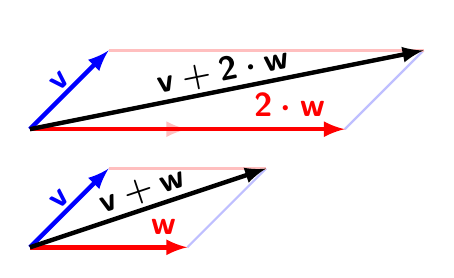
\begin{tikzpicture}[font=\boldmath]\large
    % Punkte
    \coordinate (A) at (0,0) {};
    \coordinate (B) at (2,0) {};
    \coordinate (C) at (1,1) {};
    \coordinate (D) at (3,1) {};

    % Draw the triangle
    \draw[thick, blue!25]  (B) -- (D) node[sloped,midway,above] {};
    \draw[thick, red!25]   (C) -- (D) node[sloped,midway,above] {};
    \draw[->, ultra thick, red,   arrows={-latex}]  (A) -- (B) node[sloped,right=-0.3cm, above] {$\mathsf{w}$};
    \draw[->, ultra thick, blue,  arrows={-latex}]  (A) -- (C) node[sloped,midway,above=-0.1cm] {$\mathsf{v}$};
    \draw[->, ultra thick, black, arrows={-latex}]  (A) -- (D) node[sloped,midway,above=-0.1cm] {$\mathsf{v+w}$};


    \begin{scope}[shift={(0,1.5)}]
    \draw[thick, blue!25]  (4,0) -- (5,1) node[sloped,midway,above] {};
    \draw[thick, red!25]   (1,1) -- (5,1) node[sloped,midway,above] {};
    \draw[->, ultra thick, red!25,   arrows={-latex}]  (0,0) -- (2,0);
    \draw[->, ultra thick, red,   arrows={-latex}]  (0,0) -- (4,0) node[sloped,right=-0.7cm,above] {$\mathsf{2 \cdot w}$};
    \draw[->, ultra thick, blue,  arrows={-latex}]  (0,0) -- (1,1) node[sloped,midway,above=-0.1cm] {$\mathsf{v}$};
    \draw[->, ultra thick, black, arrows={-latex}]  (0,0) -- (5,1) node[sloped,midway,above=-0.1cm] {$\mathsf{v+2 \cdot w}$};
    \end{scope}
\end{tikzpicture}
\end{document}
